\section{Experimentos y análisis de resultados}
	
	\subsection{Procedimiento de desarrollo de la práctica}
	
	\paragraph{}Para realizar la práctica, se ha optado por implementar las heurísticas propuestas en el lenguaje de programación \textsc{Java}. El ejecutable que se entrega junto a este documento ha sido compilado bajo \textsc{ Apache NetBeansIDE 12.0}.
	
	\subsubsection{Equipo de pruebas}
	
	\paragraph{}Los resultados de las heurísticas han sido obtenidos en el siguiente equipo:
	
		\begin{itemize}
			
			\item Host: 80WK Lenovo Y520-15IKBN
			\item S.O: KDE neon User Edition 5.20 x86 64
			\item Kernel: 5.4.0-52-generic
			\item CPU: Intel i5-7300HQ (4) @ 3.500GHz
			\item GPU: NVIDIA GeForce GTX 1050 Mobile
			\item GPU: Intel HD Graphics 630
			\item Memoria RAM : 7837 MiB.
			
		\end{itemize}

	\subsubsection{Manual de usuario}
	
		\paragraph{}Para ejecutar el software asegúrese de que el archivo .jar proporcionado se ubica en el mismo directorio que la carpeta \emph{archivos}. 
		
		\paragraph{}Cuando se muestre la GUI, podrá seleccionar la heurística que desee mediante el botón correspondiente. Una vez empiece la ejecución de una heurística no sera posible seleccionar otra hasta que finalice su ejecución. Los resultados finales se mostrarán en el cuadro de texto, a su vez, se generan los log correspondientes a cada archivo y semilla en la carpeta Log.
	
		\begin{figure}[H]
		
			\centering
			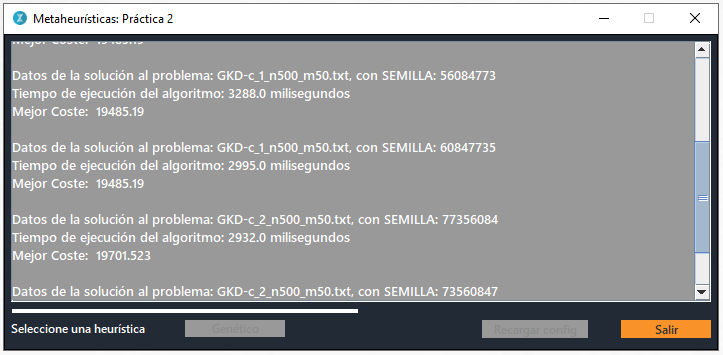
\includegraphics[scale=0.4]{img/GUI}
			\caption{GUI}
		
		\end{figure}
	
	\subsection{Parámetros de los algoritmos}
	
		\subsubsection{Genetico}


	
	\subsubsection{Semillas}
	
	\paragraph{}Para la generación de números pseudoaleatorios se utiliza una semilla previamente definida en el archivo de configuración, en este caso es 77356084. Esta semilla se va rotando en las 5 iteraciones de cada archivo.
	
	
	\paragraph{} 77356084 $\rightarrow$ 73560847 $\rightarrow$ 35608477  ...
	
	
	\subsection{Análisis de los resultados}
	
	\subsubsection{Efectos de la mutación}
	
	\paragraph{} La mutación en los algoritmos genéticos es una técnica de diversificación, la cual puede ayudar a salir de óptimos locales, no obstante, su porcentaje de aplicación debe ser reducido.Esto es debido a que una alta probabilidad de mutación puede alterar considerablemente las soluciones obtenidas, resultando en una calidad inferior de las mismas.
	
	 Para reflejar este comportamiento de la mutación, se ha seleccionado el conjunto de datos SOM, y se ha establecido 3 valores distintos de probabilidad de mutación: 0,01, 0,05 y 0,09. Cada Probabilidad de mutación se ha aplicado en 5 iteraciones, con distinta semilla para cada archivo. Posteriormente se ha obtenido la media de las 5 iteraciones para cada archivo y probabilidad de mutación, de dichos resultados se ha obtenido la siguiente gráfica:
	 
		 \begin{figure}[H]
		 	
		 	\centering
		 	\includegraphics[scale=0.6]{img/Mutación}
		 	\caption{Diferencias en porcentajes respecto a los óptimos globales}
		 	
		 \end{figure}
	 
	 \paragraph{}Como se puede observar, un mayor porcentaje de mutación, empeora los resultados obtenidos mediante algoritmos genéticos.
	
	\paragraph{} 
	
